\documentclass[tikz]{standalone}%

\usepackage[utf8]{inputenx}%  http://ctan.org/pkg/inputenx
% Euler for math | Palatino for rm | Helvetica for ss | Courier for tt
\renewcommand{\rmdefault}{ppl}% rm
\linespread{1.05}% Palatino needs more leading
\usepackage[scaled]{helvet}% ss //  http://ctan.org/pkg/helvet
\usepackage{courier}% tt // http://ctan.org/pkg/courier
\usepackage{eulervm}  %  http://ctan.org/pkg/eulervm
% a better implementation of the euler package (not in gwTeX)
\normalfont%
\usepackage[T1]{fontenc}%  http://ctan.org/pkg/fontenc
\usepackage{textcomp}%  http://ctan.org/pkg/textcomp

\usetikzlibrary{angles}
\usetikzlibrary{quotes}

\begin{document}
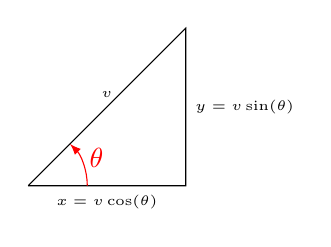
\begin{tikzpicture}
  \coordinate (A) at (0, 0);
  \coordinate (B) at (2, 0);
  \coordinate (C) at (2, 2);

  \draw (A) -- (B) node[font = \tiny, pos = 0.5, below] {$x = v\cos(\theta)$}
   -- (C) node[font = \tiny, pos = 0.5, right] {$y = v\sin(\theta)$}
   -- (A) node[above, pos = 0.5, font = \tiny] {$v$}
   pic["$\theta$", draw, -latex, angle radius = .75cm,
   angle eccentricity = 1.25, red] {angle = B--A--C};
\end{tikzpicture}
\end{document}
%%% Local Variables:
%%% mode: latex
%%% TeX-master: t
%%% End:
